%%%%%%%%%%%%%%%%%%%%%%%%%%%%%%%%%%%%%%%%%
% Stylish Article
% LaTeX Template
% Version 2.1 (1/10/15)
%
% This template has been downloaded from:
% http://www.LaTeXTemplates.com
%
% Original author:
% Mathias Legrand (legrand.mathias@gmail.com) 
% With extensive modifications by:
% Vel (vel@latextemplates.com)
%
% License:
% CC BY-NC-SA 3.0 (http://creativecommons.org/licenses/by-nc-sa/3.0/)
%
%%%%%%%%%%%%%%%%%%%%%%%%%%%%%%%%%%%%%%%%%

%----------------------------------------------------------------------------------------
%	PACKAGES AND OTHER DOCUMENT CONFIGURATIONS
%----------------------------------------------------------------------------------------

\documentclass[fleqn,10pt]{SelfArx} % Document font size and equations flushed left

\usepackage{subcaption}
\usepackage[english]{babel} % Specify a different language here - english by default
\usepackage{array,booktabs}% http://ctan.org/pkg/{array,booktabs}
\usepackage{lipsum} % Required to insert dummy text. To be removed otherwise
\usepackage[section]{placeins}
\usepackage{amsmath}
\newcolumntype{P}[1]{>{\centering\arraybackslash}p{#1}}
\newcolumntype{M}[1]{>{\centering\arraybackslash}m{#1}}
%----------------------------------------------------------------------------------------
%	COLUMNS
%----------------------------------------------------------------------------------------

\setlength{\columnsep}{0.55cm} % Distance between the two columns of text
\setlength{\fboxrule}{0.75pt} % Width of the border around the abstract

%----------------------------------------------------------------------------------------
%	COLORS
%----------------------------------------------------------------------------------------

\definecolor{color1}{RGB}{0,0,90} % Color of the article title and sections
\definecolor{color2}{RGB}{0,20,20} % Color of the boxes behind the abstract and headings

%----------------------------------------------------------------------------------------
%	HYPERLINKS
%----------------------------------------------------------------------------------------

\usepackage{hyperref} % Required for hyperlinks
\hypersetup{hidelinks,colorlinks,breaklinks=true,urlcolor=color2,citecolor=color1,linkcolor=color1,bookmarksopen=false,pdftitle={Title},pdfauthor={Author}}

%----------------------------------------------------------------------------------------
%	ARTICLE INFORMATION
%----------------------------------------------------------------------------------------

\JournalInfo{\today} % Journal information
\Archive{} % Additional notes (e.g. copyright, DOI, review/research article)

\PaperTitle{{\small ESE650 Project 2:} \\Orientation Tracking using Unscented Kalman Filter} % Article title

\Authors{Nischal K N\\nischal@seas.upenn.edu} % Authors
%\affiliation{\textsuperscript{1}\textit{Department of Biology, University of Examples, London, United Kingdom}} % Author affiliation
%\affiliation{\textsuperscript{2}\textit{Department of Chemistry, University of Examples, London, United Kingdom}} % Author affiliation
%\affiliation{*\textbf{Corresponding author}: john@smith.com} % Corresponding author

\Keywords{} % Keywords - if you don't want any simply remove all the text between the curly brackets
\newcommand{\keywordname}{Keywords} % Defines the keywords heading name

%----------------------------------------------------------------------------------------
%	ABSTRACT
%----------------------------------------------------------------------------------------

\Abstract{Tracking the pose of a body helps to understand the attitude of the object in the world frame. Few of such sensors used for attitude tracking accelerometer, gyroscope, magnetometer, barometer, etc. But however each of these sensors are not perfect and have to be filtered or combined to produce a sensible output. This project discusses a few methods and their results., namely Kalman filter and complementary filter for determining the orientation of an object in the world frame.}

%----------------------------------------------------------------------------------------

\begin{document}

\flushbottom % Makes all text pages the same height

\maketitle % Print the title and abstract box

\tableofcontents % Print the contents section

\thispagestyle{empty} % Removes page numbering from the first page

%----------------------------------------------------------------------------------------
%	ARTICLE CONTENTS
%----------------------------------------------------------------------------------------
\section{Introduction}
In this project, data from accelerometer and gyroscope of an IMU are used together to determine the orientation of the body in the world frame. Each sensor accelerometer and gyroscope information individually can be used to obtain the orientation information but however they have some drawbacks. The gyro drifts over time. That means it can not be trusted for a longer time spans, but it is very precise for a short time. This is when the accelerometer comes in handy. It does not have any drift, but it is too unstable for shorter time spans. A complementary filter and an unscented kalman filter is implemented to mix these measurements and the results are compared. The advantage of unscented kalman filter is that it operates on a non linear state and does not approximate it to a linear system. As a result it can capture the attitude much better. The report is divided as follows. Section \ref{sec:dataset} explains the dataset, Section \ref{sec:acc} and \ref{sec:gyro} gives the results of determining the orientation with accerometer and gyroscope alone and also discusses their shortcomings. Section \ref{sec:comp} discusses the results of complementary filter and Section \ref{sec:ukf} explains how unscented kalman filter was implemented. 

\section{Dataset}
\label{sec:dataset}
The dataset consists of 9 sets of raw imu 10bit ADC readings for approximately 30sec to 60sec of motion. The motion is restricted to rotation and limited translation. Each dataset consists of different series of motion. This motion is also captured by the vicon system which is used as a ground reference. The vicon data is in the from of a rotation matrix. Also camera image is provided to stitch a panorama based on the filter output. Each of this data is accopanied by its corresponding time stamp.

\section{Orientation using accelerometer}
\label{sec:acc}
The acelerometer data is three 10bit ADC values representing the accelratin in 3 directions. The earths gravity component is split into the 3 axis components. When placed stationary and parrel to the ground, the accelerometer must read 0 on x axis, 0 on y axis and 9.81 on z axis. But however the output contains a lot of bias and also has to be scaled. This can be done by using the ground truth obtained from the vicon system.

\begin{figure*}[t]
\centering
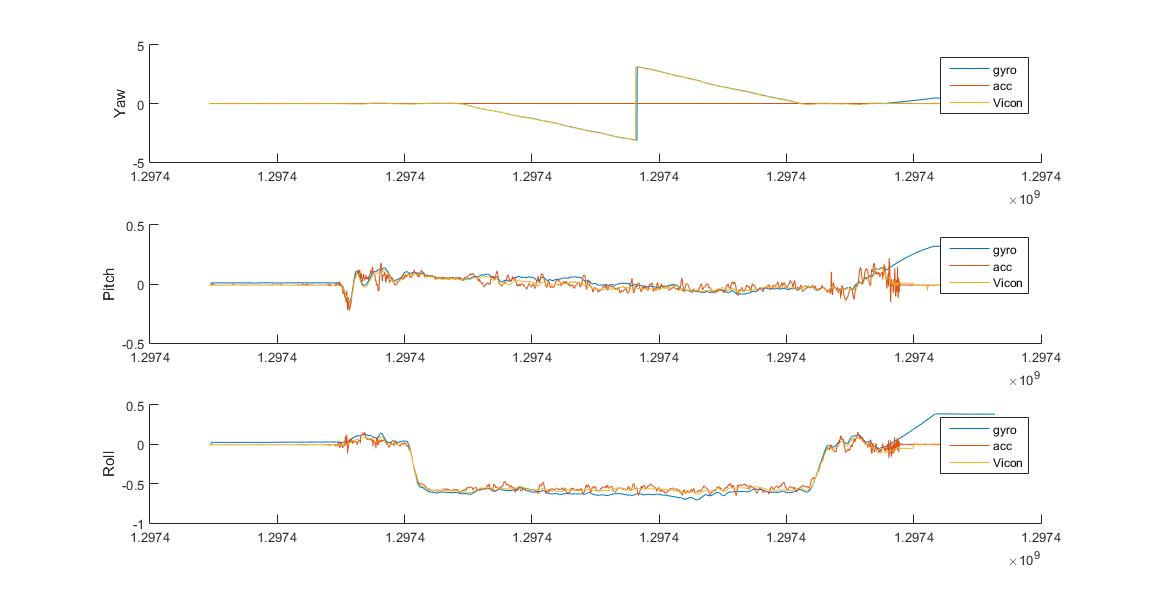
\includegraphics[scale=0.4]{raw.jpg}
\caption{Orientation Estimate using Gyroscope and accelerometer for test set}
\label{fig:raw}
\end{figure*}

\subsection{Scale and bias}
To bring the IMU readings from world frame to body frame, we rotate the vicon rotation matrix with [0;0;9.81]. Then it is compared with the accelerometer readings keeping bias and scale as variables. Multiple simultaneous equations are solved to obtain the scale and bias values for each axis. The matrix representation of the simultaneous equations are shown below.
\begin{align*}
 \begin{bmatrix}
    a_{x1} & 1 \\
    a_{x1} & 1 \\
    \vdots & \vdots \\
    a_{xn} & 1 \\
  \end{bmatrix}
  *&
\begin{bmatrix}
    S \\
    B
  \end{bmatrix} 
  =
  \begin{bmatrix}
    gx_1' \\
    gx_2' \\
    \vdots \\
    gx_n' \\
  \end{bmatrix} \\
\intertext{Where $a_{x1},a_{x2},\ldots,a_{xn}$ are x axis readings of accelerometer, $S$ is the best fit scale, $B$ is the best fit bias and $g'$ is given as}
g' =
\begin{bmatrix}
    gx \\
    gy \\
    gz \\
 \end{bmatrix}
  =&\; R*  
\begin{bmatrix}
    0 \\
    0 \\
    1 \\
 \end{bmatrix}
\end{align*}
and $gx_1,gx_2,\ldots,gx_n$ are the x values of $g'$ for all samples.
Another way to calculate the scale of an accelrometer is by using the sensitivity information from the datasheet
\begin{align*}
scale =&\; Vref/1023 * sensitivity
\intertext{The final accelerometer value is obtained by}
acc =&\; scale*raw - bias;
\end{align*}

\subsection{Orientation estimation}
To obtain the orientation with the accelerometer alone we take the $tan^{-1}$ of the respective components. However we can get only roll and pitch from accelerometer and not yaw. The roll($\theta$) and pitch($\phi$) are given by \cite{acce}

\begin{align*}
\theta =&\; \tan^{-1} \frac{A_x}{\sqrt{A_y^2+A_z^2}} \\
\phi =&\; \tan^{-1} \frac{A_y}{\sqrt{A_x^2+A_z^2}}
\end{align*}

The orientation estimate using accelerometer alone is shown in red in Fig. \ref{fig:raw}. The estimation is pretty noisy.

\section{Orientation using gyroscope}
\label{sec:gyro}
Gyroscope measures angular velocity and outputs three 10bit ADC values representing angular velocity along each axis. Again like accelerometer, the readings have a bias and a scale factor in them. They have to be compensated before it can be used.
\subsection{Bias and Scale estimation}
To compute the bias of the gyro, the intial 200 samples of each dataset is used. The average of all these values in each axis gives the bias of each axis. This is because, initially the body is stationary and the angular velocity is ideally zero. Any value recorded by the sensor is the bias. To calculate the scale, the information about sensitivity from the datasheet is used
\begin{align*}
scale = \frac{Vref}{1023} * \frac{pi}{180*sensitivity}
\intertext{This is used to obtain the corrected gyroscope values}
gyro = (raw-bias) * scale
\end{align*}

\subsection{Orientation estimation}
The orientation of the body can be obtained from the gyroscope readings alone by integrating over time. But however since gyroscope drift overtime, it is inaccurate over long periods. Since the orientation is estimated by integration, the error keeps accumulating and finally becomes unusable.
\begin{align*}
\theta =&\; \int_{0}^{t}G_x dt \\
\phi =&\; \int_{0}^{t}G_y dt \\
\varphi =&\; \int_{0}^{t}G_z dt
\end{align*}
The orientation estimate of gyroscope with respect to vicon is shown in blue in Fig. \ref{fig:raw}. It is seen that it drifts a lot during the end.

\section{Complimentary Filter}
\label{sec:comp}
In the above sections we have seen that the accelrometer is unstable over small intervals as it measures all forces that are working on the object, it will also see a lot more than just the gravity vector and also cannot measure yaw and gyroscope drift over time and accumulates error making it unusable over longer durations. To get the best of both worlds, we use complimentary filter which takes a weighted average of both measurements. The roll($\theta$), pitch($\phi$) and yaw($\varphi$) is given as
\begin{align*}
\theta =&\; W_g \times (\theta + \int_{0}^{t}G_x dt) + W_a \times \tan^{-1} \frac{A_x}{\sqrt{A_y^2+A_z^2}} \\
\phi =&\; W_g \times (\phi + \int_{0}^{t}G_y dt) + W_a \times \tan^{-1} \frac{A_y}{\sqrt{A_x^2+A_z^2}}\\
\varphi =&\; (\varphi + \int_{0}^{t}G_z dt)
\end{align*}
Where $W_g$ is the weight given to the gyro readings and $W_a$ is the weight given to the accelerometer. Since yaw is not measured reliably by accelerometer, it is not used to determine yaw. The output of this can be seen in Fig. \ref{fig:com_g} and Fig. \ref{fig:com_b}. Fig. \ref{fig:com_g} is the complementary filter output for the set set. It is seen that it estimates the orientation quite accurate, but however it fails over time due to drift in gyro as seen in Fig. \ref{fig:com_b}. To conclude complimentary filter does low pass filter on accelerometer readings and high pass filter on gyro readings.

\section{UKF}
\label{sec:ukf}
An Unscented Kalman Filter is an extension of Kalman filter which preserves the non linear state of the model. This performs better than kalman filter when there is a non linear state update function because of the linear approximation done by kalman filter. UKF uses a deterministic sampling technique called unscented transformt to pick sample points called sigma points and keeps track of them as they propagate through states. The mean and covariance of the state distribution is also calculated from them. The following is the algorithm used in the implementation of this project

\begin{figure}[h]
\centering
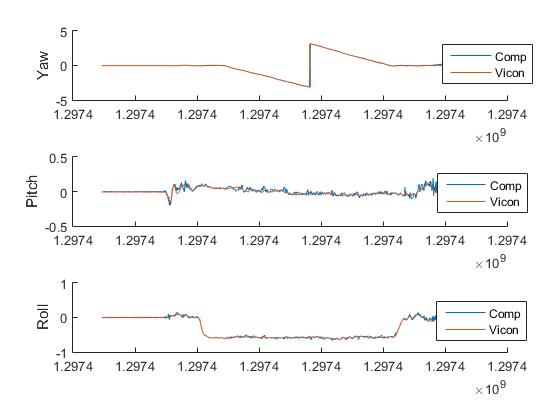
\includegraphics[scale=0.45]{com_good.jpg}
\caption{Complimentary filter for test set}
\label{fig:com_g}
\end{figure}

\begin{figure}[h]
\centering
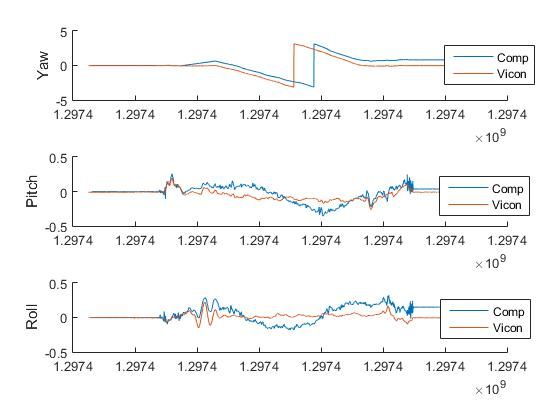
\includegraphics[scale=0.45]{com_bad.jpg}
\caption{Complimentary filter for dataset 9}
\label{fig:com_b}
\end{figure}

\begin{enumerate}
\item The state of the system is initialized by a initial state vector $x_0$ which consists of the quaternion($q$) part and a angular velocity($\omega$) part. The initial covariance(P), process noise(Q) and measurement noise(R) are also initiate. The noise Q and R have to be tuned.
\[
x_o = \begin{matrix}
q \\ \vec{w}
\end{matrix}
\]
In this project the Process noise and measurement noise were
\begin{align*}
Q =&\; diagonal(78.97,78.97,78.97,6.5,6.5,6.5) \\
R =&\; diagonal(0.2,0.2,0.2,3,3,3)
\end{align*}
\item The sigma points are chosen from the Cholesky decomposition of P+Q and then multiplying by a scale factor of $sqrt(n)$ \cite{Julier}. The sigma points $\chi_i$ are given by
\begin{align*}
S =&\; \sqrt{P_{k-1}+Q} \\
W =&\; columns(\pm\sqrt{n}*S) \\
\chi_i =&\; x_{k-1} + W \\
=&\; \begin{bmatrix}
q_{k-1}q_W \\
\vec{\omega}_{k-1}+\vec{\omega}_W
\end{bmatrix}
\end{align*}
\item The process model update is a non linear function of the sigma points, which project each point ahead of time. It is given as
\begin{align*}
Y =&\; A(\chi_i,0) \\
=&\; \begin{bmatrix}
q_{k-1}q_Wq_\Delta \\
\vec{\omega}_{k-1}+\vec{\omega}_W
\end{bmatrix}
\intertext{where,}
q_\Delta =&\; \begin{bmatrix}
cos(\frac{\alpha_\Delta}{2}) & \vec{e}_\Delta sin(\frac{\alpha_\Delta}{2})
\end{bmatrix}
\end{align*}
\item The mean($\bar{x}_k$) of the distribution is found out by intrinsic gradient decent of the sigma point as explained in \cite{Kraft}. To initialize the gradient decent the previous mean is used to allow faster convergence. The covariance($P_k$) is found out as follows
\begin{align*}
\hat{\bar{x}}_k =&\; mean(Y_i) \\
P_k =&\; \frac{1}{2n}\sum_{i=1}^{2n}[\chi_i - \hat{\bar{x}}_k][\chi_i - \hat{\bar{x}}_k]^\top
\end{align*}
\item The measurement model update is performed using another non linear function on the transformed sigma points so that it can applied on the measured values. The measurements update model for gyro is $H_1$ and accelrometer is $H_2$
\begin{align*}
Z_i =&\; H(Y_i,0) \\
H_1 =&\; \vec{\omega_k} \\
H_2 =&\; g' = q_kgq_k^{-1} \\
\therefore Z_i =&\; \begin{bmatrix}
q_kgq_k^{-1} \\
\vec{\omega_k}
\end{bmatrix}
\end{align*}
\item The mean and projected state vector covariance is found as follows
\begin{align*}
\bar{z_k} =&\; \frac{1}{2n}\sum_{i=1}^{2n} Z_i \\
P_{zz} =&\; \frac{1}{2n}\sum_{i=1}^{2n}[Z_i-\bar{z_k}][Z_i-\bar{z_k}]^\top
\end{align*}
\item The innovation term is the difference between the process model and the actual measurements given by
\[
v_k = z_k - \bar{z_k}
\]
\item The expected covariance of the innovation term is the sum of $P_{zz}$ and measurement noise R.
\[
P_{vv} = P_{zz} +  R
\]
\item The cross-corelation matrix $P_{xz}$ relates the noise in the state vector to the noise in the measurement.
\[
P_{xz} = \frac{1}{2n}\sum_{i=1}^{2n}[Y_i-\hat{\bar{x}}_k][Z_i-\bar{z_k}]^\top
\]
\item The kalman gain of the UKF is calculated as
\[
K_k = P_{xz}P^{-1}_{vv}
\]
\item The state equation update of the posteriori estimate is
\begin{align*}
\hat{x}_k =&\; \bar{\hat{x}}_k + K_kv_k \\
P_k =&\; \bar{P}_k - K_kP_{vv}K_k^\top
\end{align*}
\end{enumerate}
One aspect noticed during the implementation process is that the system is highly susceptible to tuning of the noise parameters Q and R. Since the measurements from gyro are stable over small period of time, the covariance is about 0.2, which is less compared to accelerometer noise which is 3.

\section{Image stitching}
Using the orientation information from the kalman filter output, a series of camera images were stitched to generate a panoromic image. The camera image that is currently in the body frame is rotated by a rotation matrix determined by the kalman filter. This converts the image into world frame. The images are synced with the imu reading through the time stamp. 2 kinds of project were performed on this. 
\begin{enumerate}
\item Initially a homographic projection of the image was done. The images were placed on a canvas based on the roll, pitch and yaw obtained from the kalman filter output. As the roll changes, the image on the canvas was rotated to keep the image upright. As pitch changed, it means the body is rotated about y axis, and the image was moved vertically on the canvas and finally as yaw changed, the image was moved horizontally. The amount of rotation of the image was equal to the negative of roll($\theta$). An arbitrary distance $d$ of the image from the camera was considered. The horizontal(H) and vertical(V) displacements of the image was calculated
\begin{align*}
H =&\; d \times tan(\phi) \\
V =&\; d \times tan(\varphi) \\
\end{align*}
\vspace{-1cm}
\item Another method experimented was cylindrical projection \cite{cyc}. The image was first converted to world frame. An arbitrary focal length $f$ was considered for cylindrical projection of the image on a canvas with centers $\hat{x}_c$ and $\hat{y}_c$. The projection of the image onto a cylinder with parameters $\theta$ and $h$ are
\begin{align*}
\theta =&\; tan^{-1}\frac{Y}{X} \\
h =&\; \frac{Z}{\sqrt{X^2+Y^2}} \\
\intertext{The images are then projected onto the canvas using}
(\hat{x},\hat{y}) =&\; (-f\theta,fh) + (\hat{x}_c,\hat{y}_c)
\end{align*}
\end{enumerate}

\section{Experiments and Results}
\label{sec:results}
The output in terms of euler angles of the estimates state from unscented kalman filter with reference to vicon position for all the training sets and the test set is shown in Fig. \ref{fig:1} to \ref{fig:10}. The panoramic stitching of images for datasets 1,2,8,9 and test set is shown in Fig. \ref{fig:pan1} to \ref{fig:pan10}.
By comparing with the outputs of other methods, namely, estimation from gyrsoscope, estiamtion from accelerometer and complementary filter it can be seen that kalman filter performs the best. The estimation from the accelerometer doesnot have an update to yaw. Also the estimate is very noisy. Whereas the gyroscope estimate is pretty accurate and provides all the three angles. But however it faces drift and becomes unstable over time. The complementary filter works well for most of the data sets, but however over extended periods of time also is susceptible to drift as seen in Fig. \ref{fig:com_b}. where is start to drift because of drift in gyroscope. But however the unscented kalman filter compensates for this drift as seen from Fig. \ref{fig:9}. \\ 

Test set euler angle output. \textbf{Fig. \ref{fig:10}}

Panorama output. \textbf{Fig. \ref{fig:pan10}}\\
The videos of panoramic image stitching is attached at

\textbf{\hyperref[https://goo.gl/fVDJEe]{https://goo.gl/fVDJEe}}
\hspace{-1cm}
\begin{figure}[hbtp]
\centering
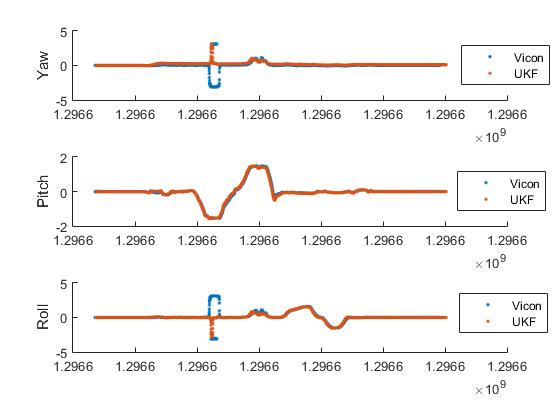
\includegraphics[scale=0.45]{1.jpg}
\caption{UKF for Training Set 1}
\label{fig:1}
\end{figure}

\begin{figure}[hbtp]
\centering
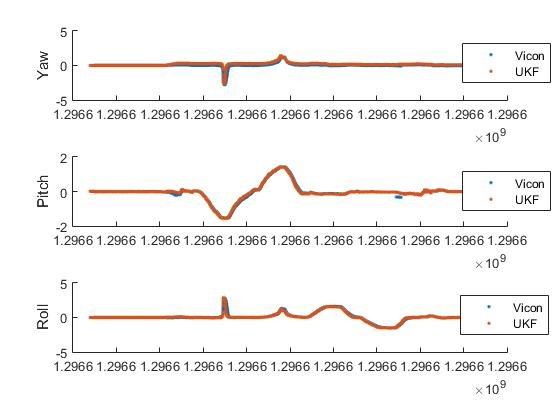
\includegraphics[scale=0.45]{2.jpg}
\caption{UKF for Training Set 2}
\label{fig:2}
\end{figure}

\begin{figure}[hbtp]
\centering
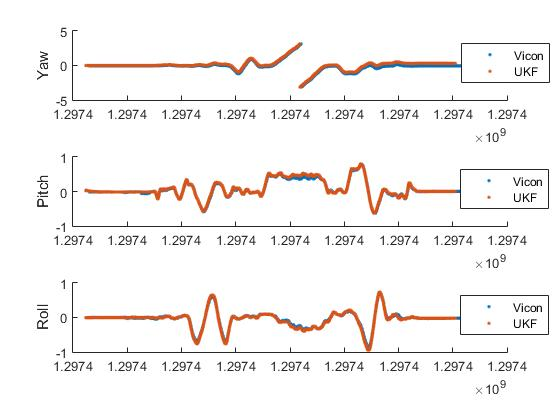
\includegraphics[scale=0.45]{3.jpg}
\caption{UKF for Training Set 3}
\label{fig:3}
\end{figure}

\begin{figure}[hbtp]
\centering
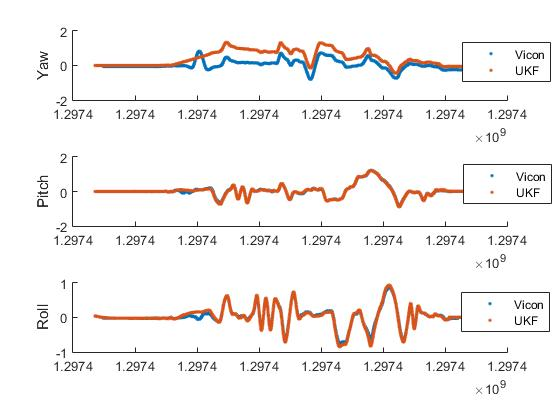
\includegraphics[scale=0.45]{4.jpg}
\caption{UKF for Training Set 4}
\label{fig:4}
\end{figure}

\begin{figure}[hbtp]
\centering
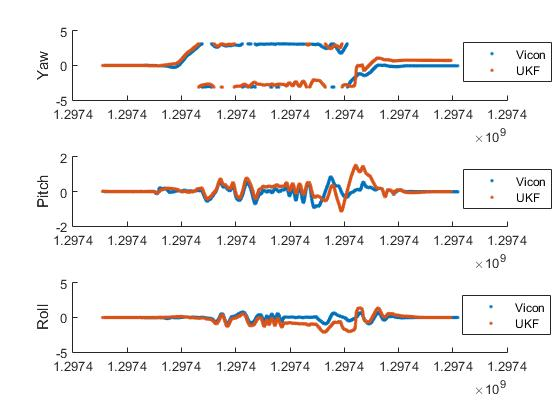
\includegraphics[scale=0.45]{5.jpg}
\caption{UKF for Training Set 5}
\label{fig:5}
\end{figure}

\begin{figure}[hbtp]
\centering
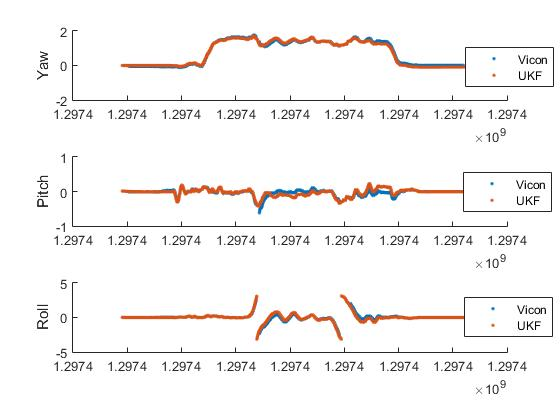
\includegraphics[scale=0.45]{6.jpg}
\caption{UKF for Training Set 6}
\label{fig:6}
\end{figure}

\begin{figure}[hbtp]
\centering
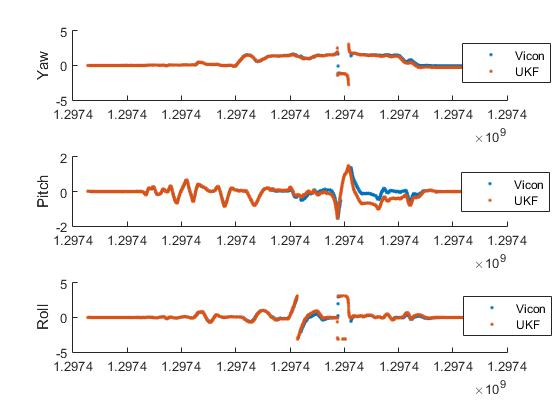
\includegraphics[scale=0.45]{7.jpg}
\caption{UKF for Training Set 7}
\label{fig:7}
\end{figure}

\begin{figure}[hbtp]
\centering
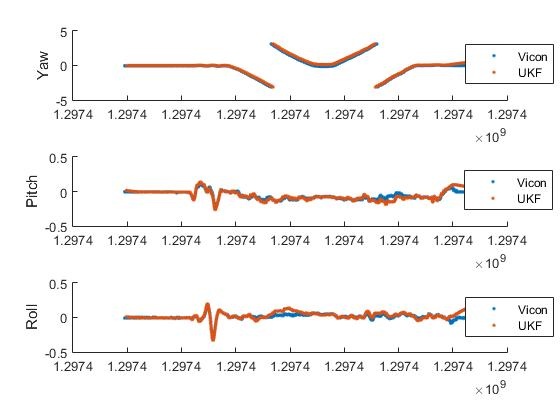
\includegraphics[scale=0.45]{8.jpg}
\caption{UKF for Training Set 8}
\label{fig:8}
\end{figure}

\begin{figure}[hbtp]
\centering
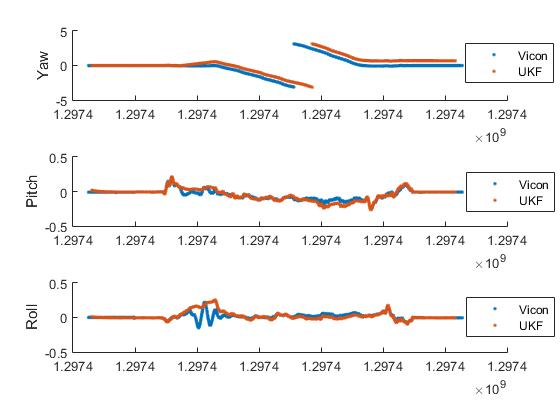
\includegraphics[scale=0.45]{9.jpg}
\caption{UKF for Training Set 9}
\label{fig:9}
\end{figure}

\begin{figure}[hbtp]
\centering
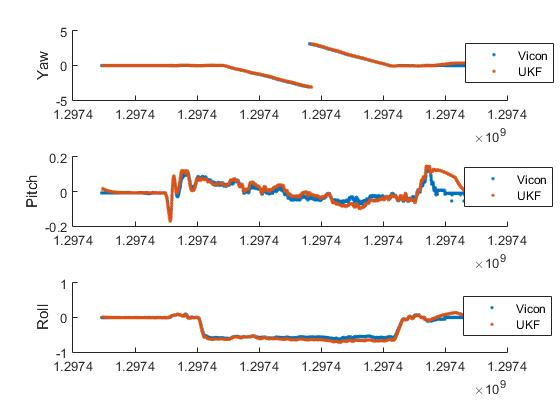
\includegraphics[scale=0.45]{10.jpg}
\caption{UKF for Test Set}
\label{fig:10}
\end{figure}

\begin{figure*}
\centering
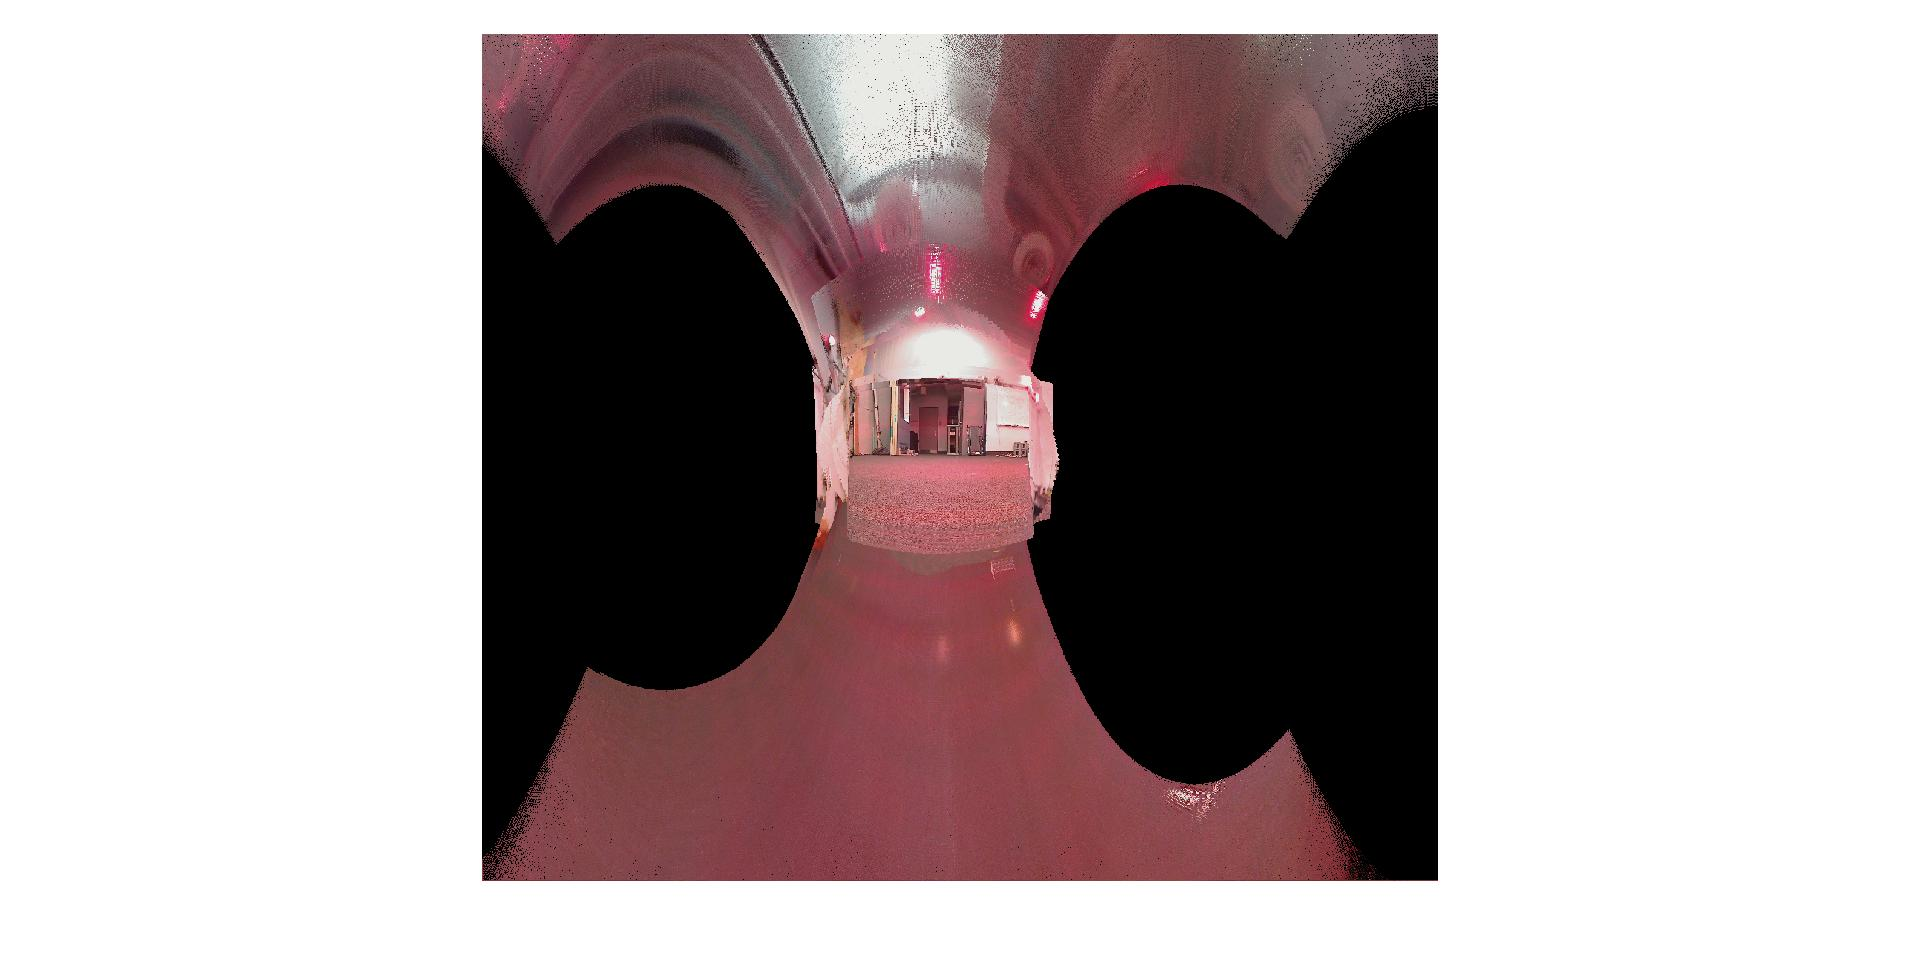
\includegraphics[trim={18cm 0cm 14cm 0cm},scale = 0.55]{pan1.jpg}
\caption{Stitched image for dataset 1}
\label{fig:pan1}
\end{figure*}

\begin{figure*}
\centering
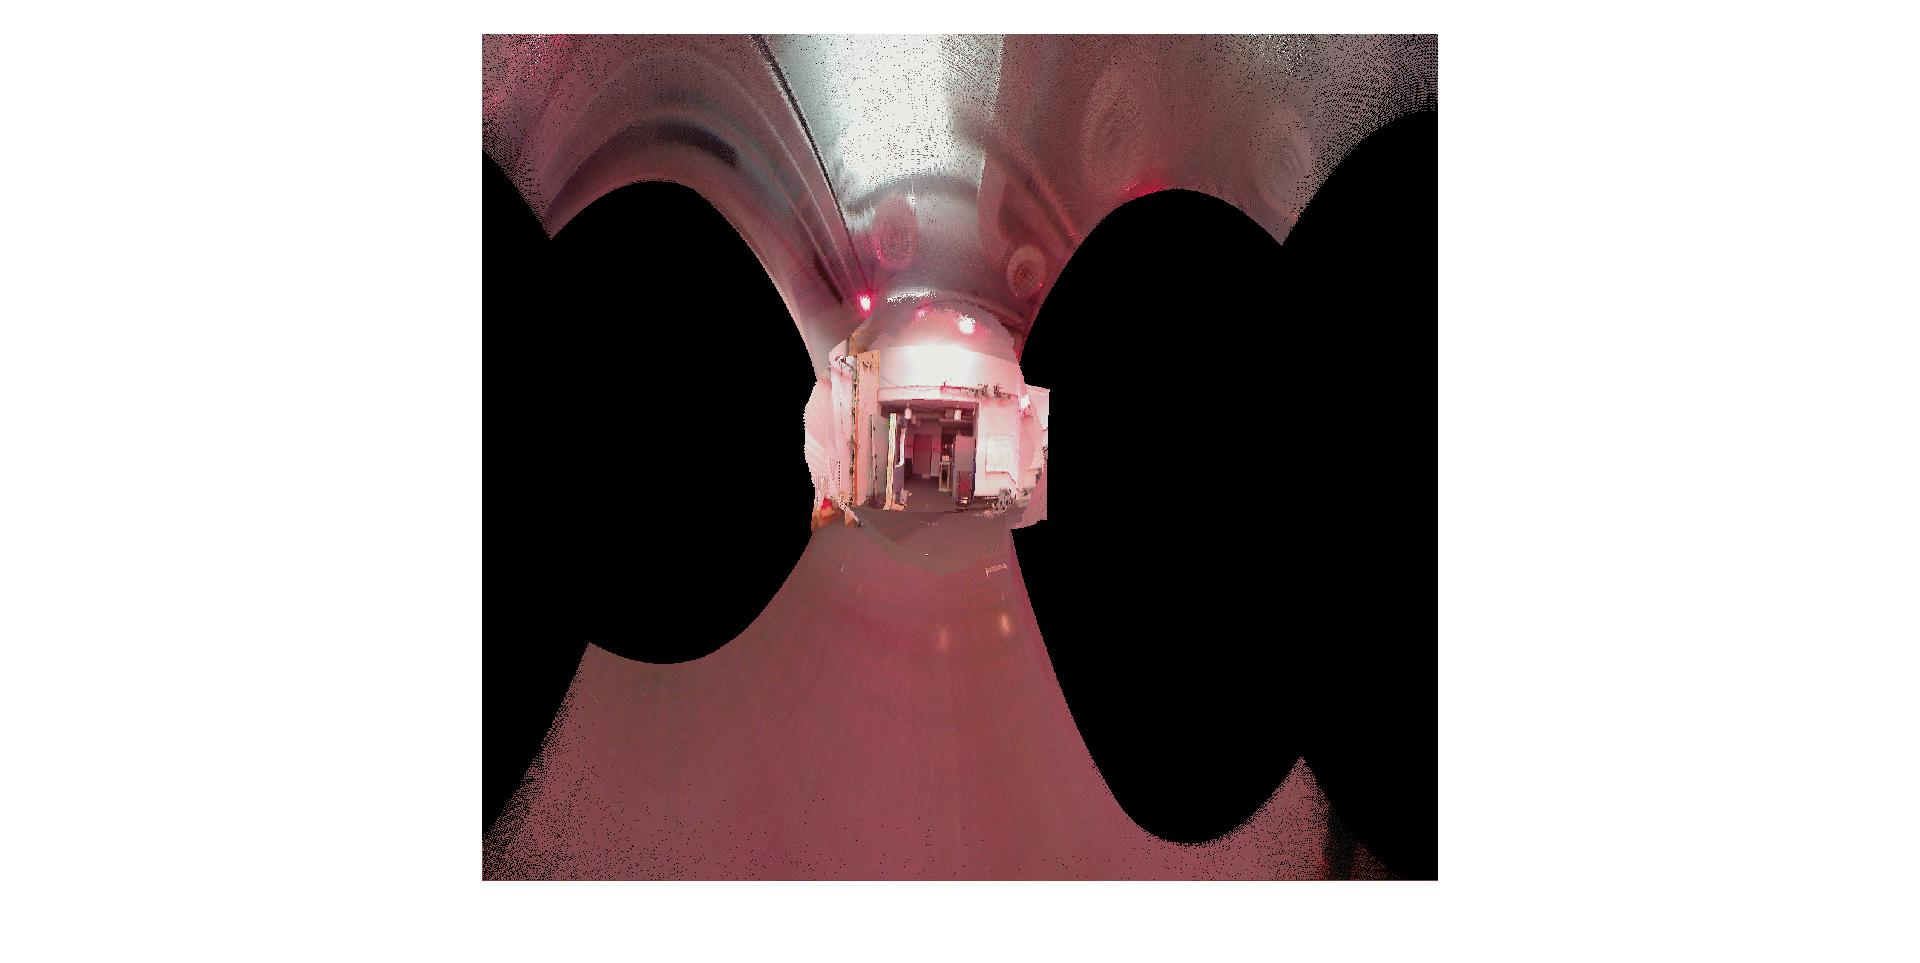
\includegraphics[trim={18cm 0cm 14cm 0cm},scale = 0.55]{pan2.jpg}
\caption{Stitched image for dataset 2}
\label{fig:pan2}
\end{figure*}

\begin{figure*}
\centering
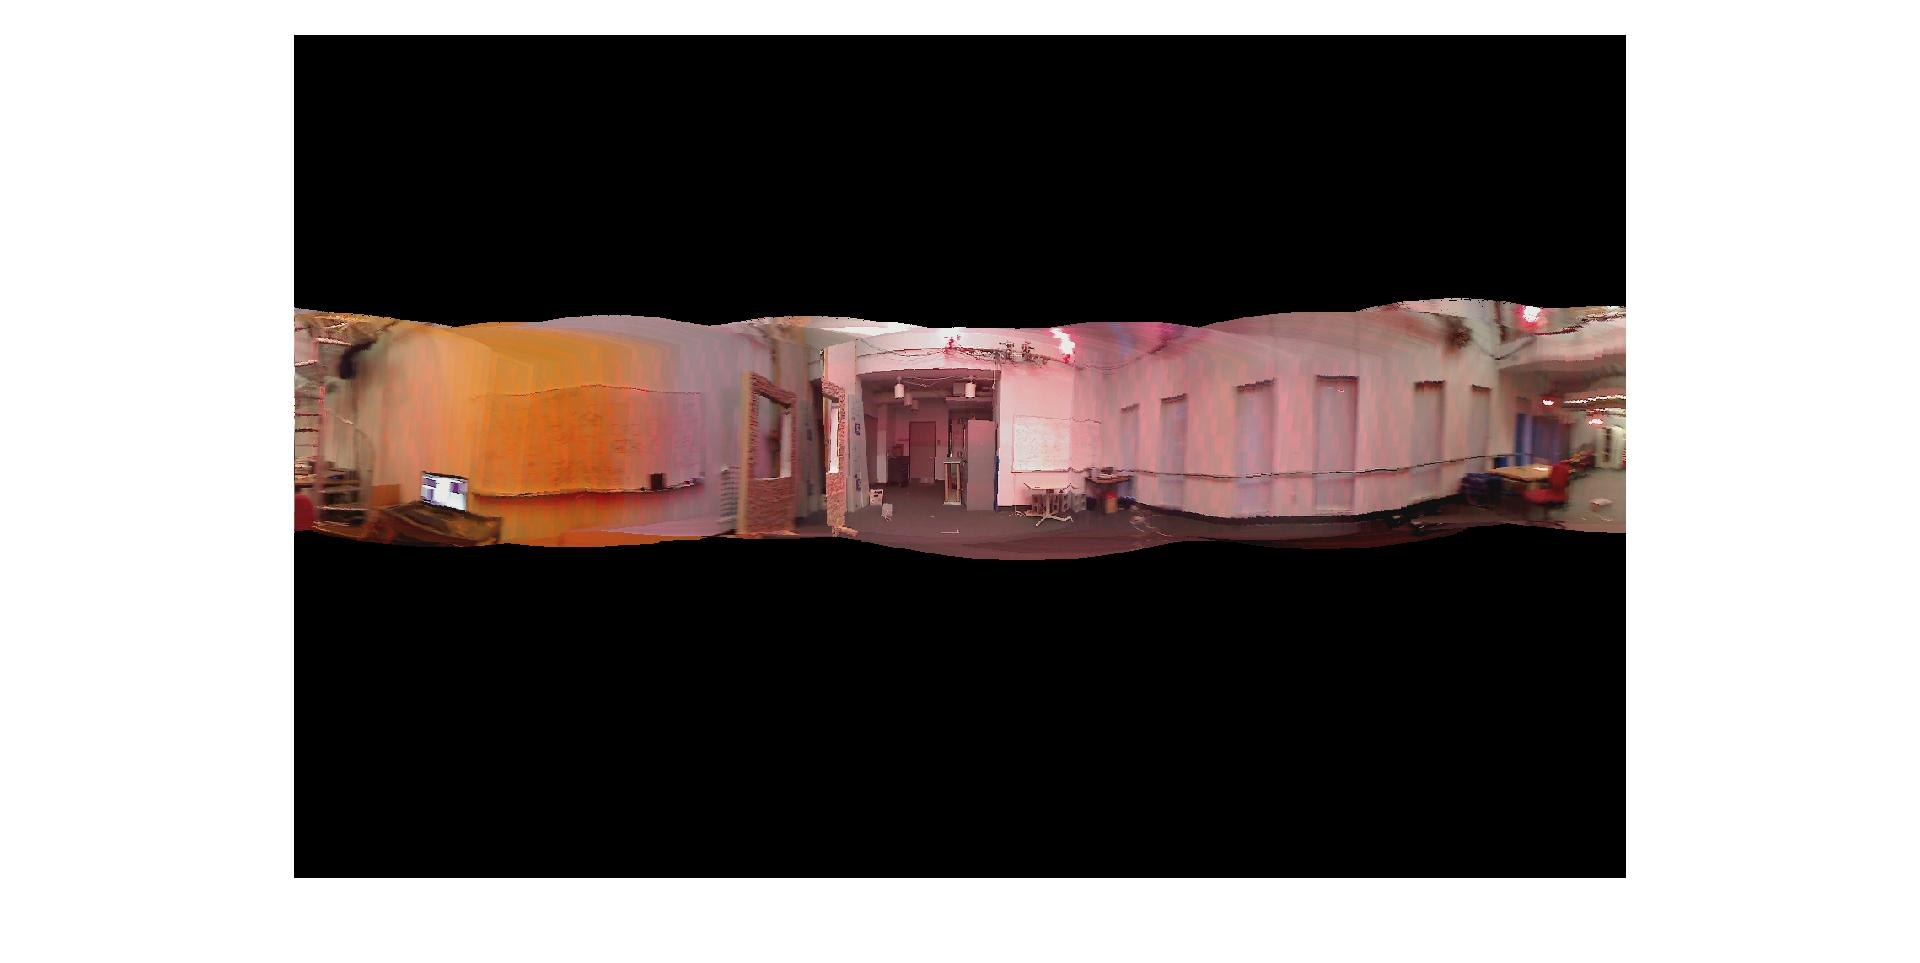
\includegraphics[trim={10cm 0cm 10cm 0cm},scale = 0.35]{pan8.jpg}
\caption{Stitched image for dataset 8}
\label{fig:pan8}
\end{figure*}

\begin{figure*}
\centering
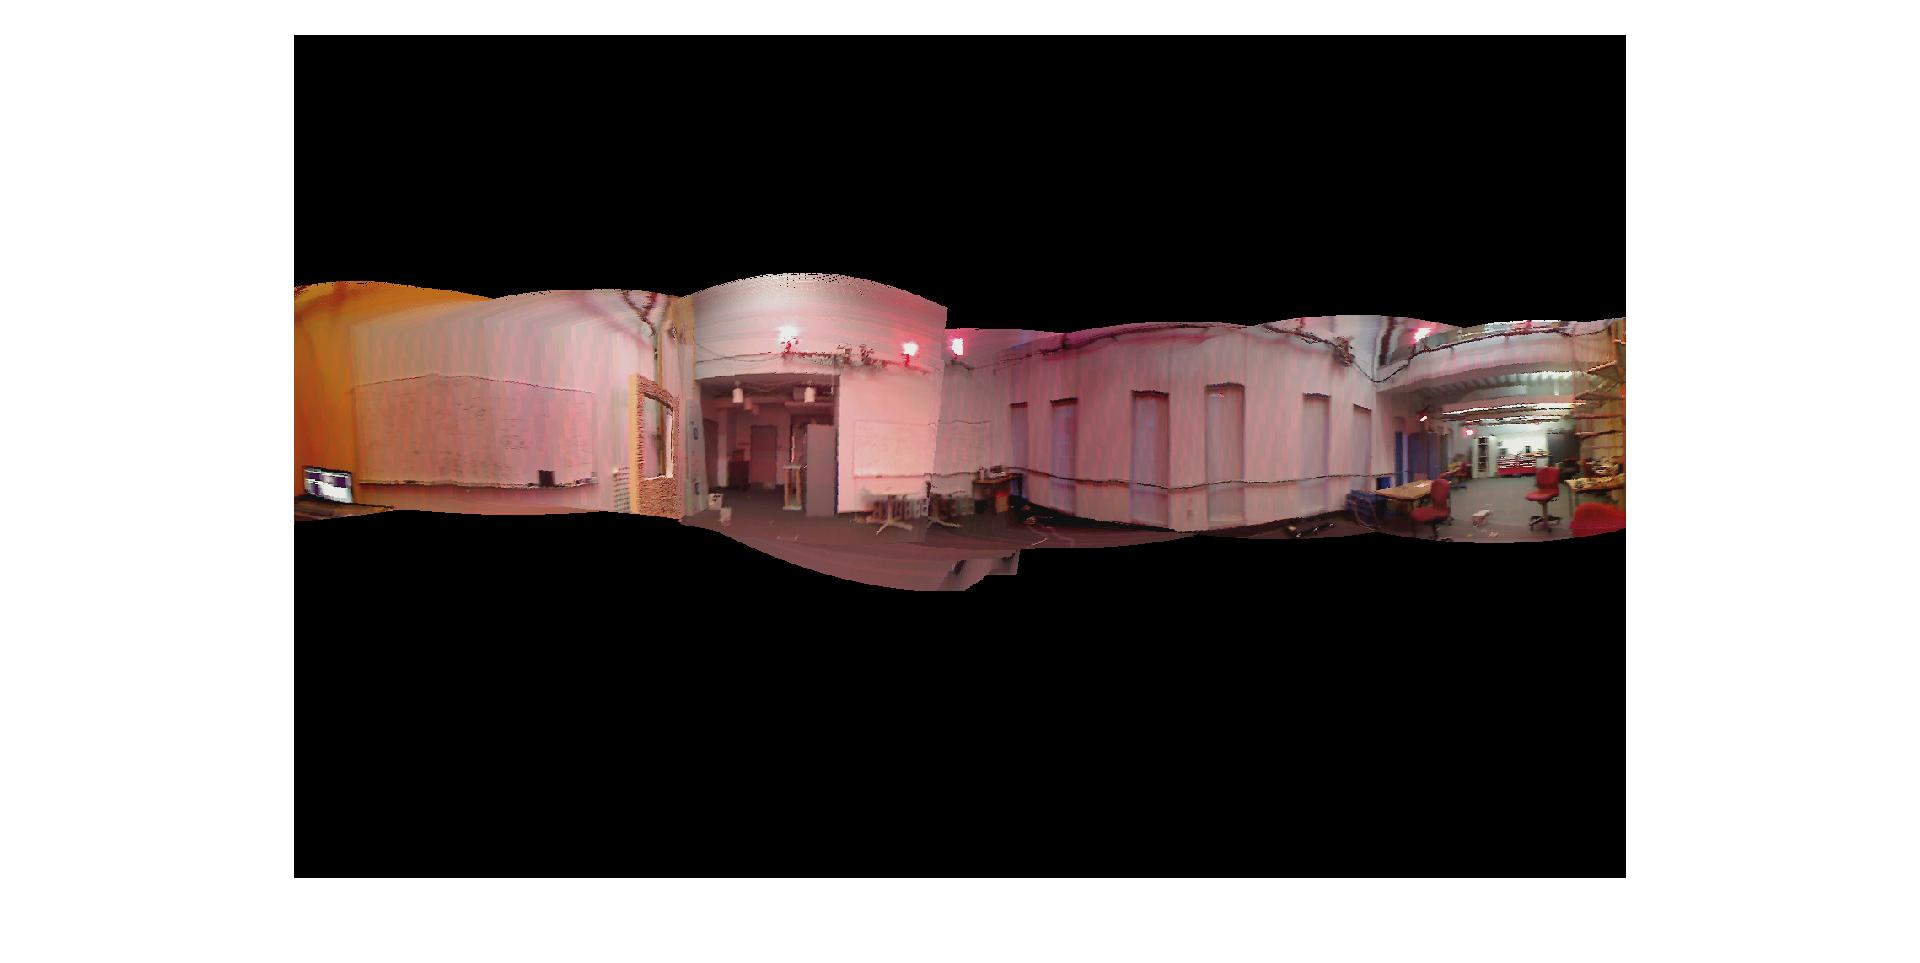
\includegraphics[trim={10cm 0cm 10cm 0cm},width=\textwidth]{pan9.jpg}
\caption{Stitched image for dataset 9}
\label{fig:pan9}
\end{figure*}

\begin{figure*}
\centering
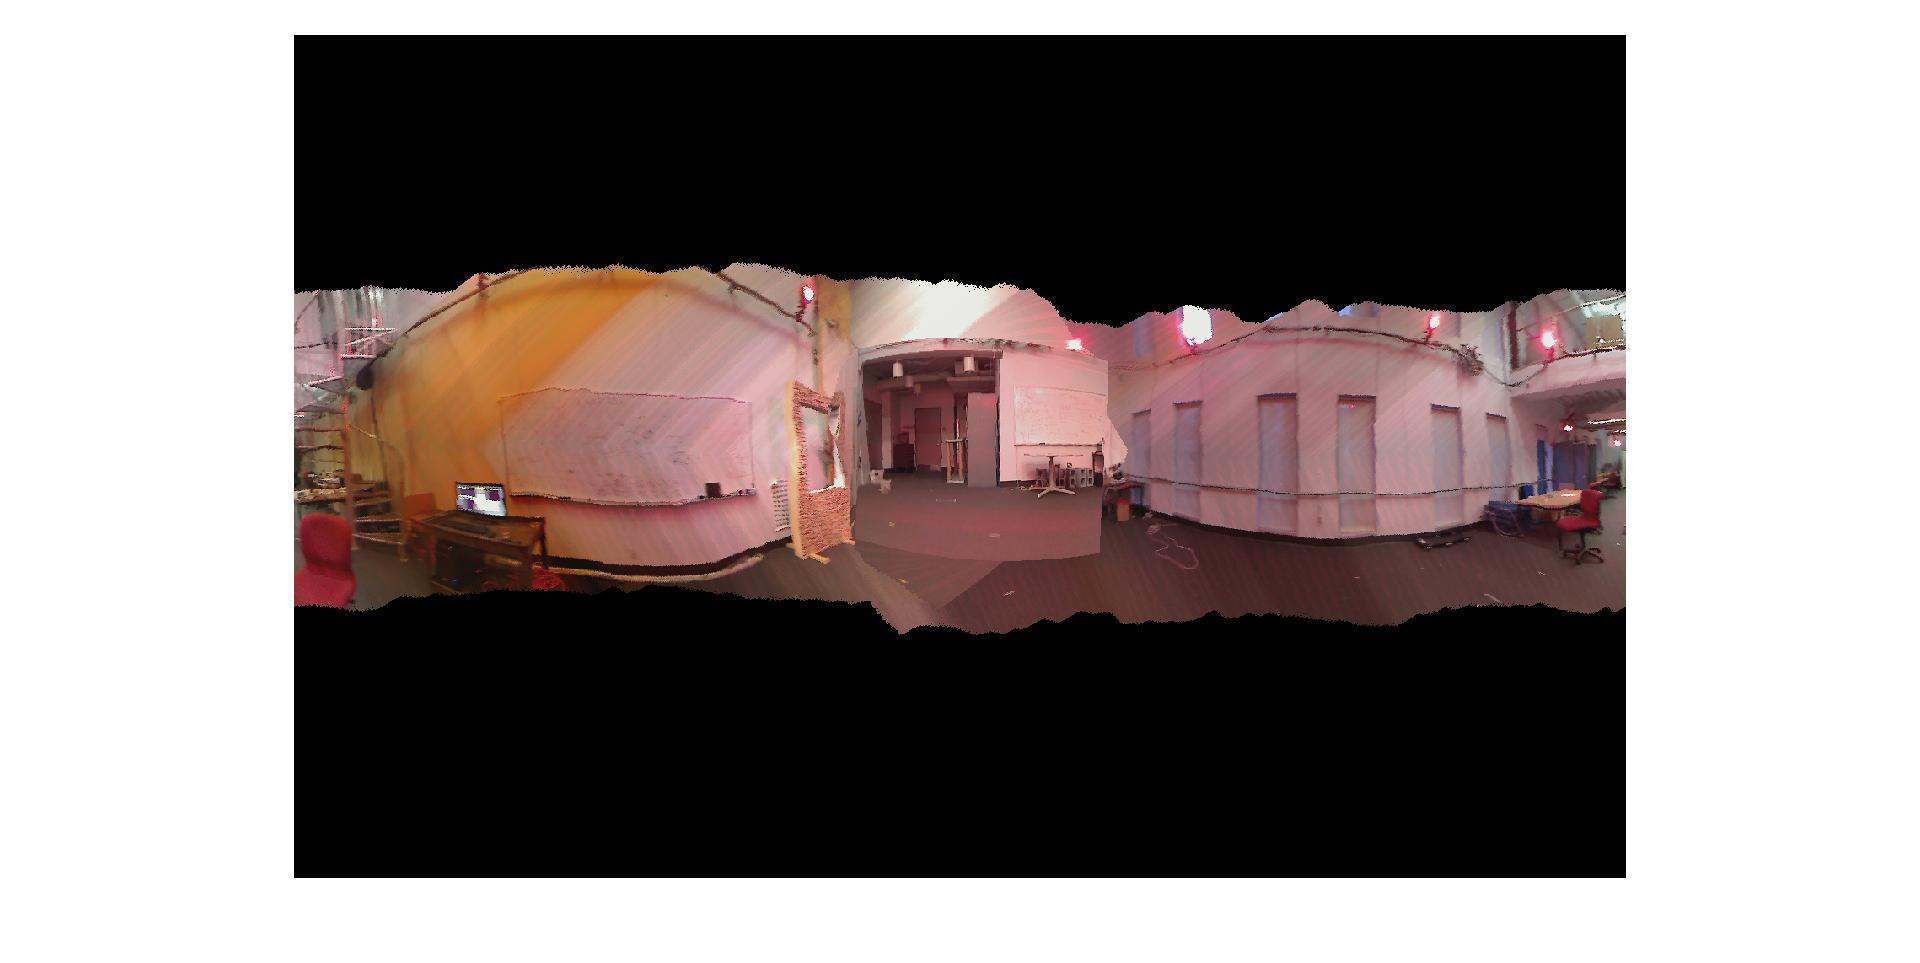
\includegraphics[trim={10cm 0cm 10cm 0cm},width=\textwidth]{pan10.jpg}
\caption{Stitched image for test set}
\label{fig:pan10}
\end{figure*}

\begin{thebibliography}{9}
\bibitem{Kraft} 
Kraft, Edgar. "A quaternion-based unscented Kalman filter for orientation tracking." Proceedings of the Sixth International Conference of Information Fusion. Vol. 1. 2003.

\bibitem{Julier}
Julier, Simon J., and Jeffrey K. Uhlmann. "New extension of the Kalman filter to nonlinear systems." AeroSense'97. International Society for Optics and Photonics, 1997.

\bibitem{acce}
\hyperref[http://www.digikey.com/en/articles/techzone/2011/may/using-an-accelerometer-for-inclination-sensing] {Using An Accelerometer for Inclination Sensing}

\bibitem{cyc}
\hyperref[http://www.csie.ntu.edu.tw/cyy/courses/vfx/05spring/lectures/handouts/lec06_stitching_4up.pdf]{Image stitching}
\end{thebibliography}

%----------------------------------------------------------------------------------------
%	REFERENCE LIST
%----------------------------------------------------------------------------------------
%\phantomsection
%\bibliographystyle{unsrt}
%\bibliography{sample}

%---------------------------------------------------------------------------------------- 

\end{document}